\section{Overview}

\bilingal{%
本章节主要描述 LGT8XM 内核构架和功能。 内核是 MCU 的大脑, 负责保证程序的正确执
行,因此内核必须能够准确的执行计算,控制外设以及处理各种中断。%
}{%
This chapter describes LGT8XM Core architecture and function. The kernel is MCU
Brain, responsible for ensuring the correct implementation of the program, so
the kernel must be able to perform accurate calculations, control peripherals
and handle a variety of interrupts.%
}

\begin{figure}[tb]
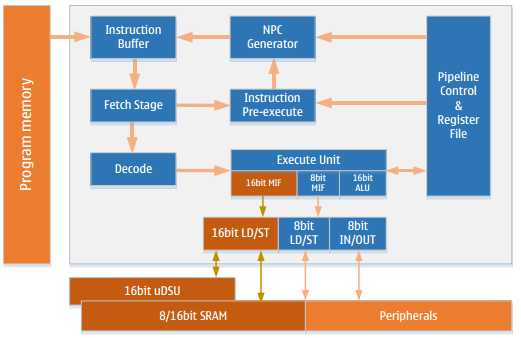
\includegraphics[width=\columnwidth]{Images/f-004}
\caption{LGT8XM core architecture.}
\end{figure}

\bilingal{%
为了实现更大的效率和并行性, LGT8XM 内核采用哈弗构架 – 独立的数据和程序总线。指
令通过一个优化的两级流水线执行,两级流水线能够减少流水线中无效指令的个数,减少了
对FLASH 程序存储器的访问量,因此可以降低内核运行的功耗。同时 LGT8XM 内核在取指令
的前级中增加了指令缓存(可以同时缓存 2 条指令),通过在取指令周期的预执行模块,
进一步减少了对FLASH 程序存储器的访问频率;经大量测试,LGT8XM 可以比其他同类构架
的内核减少约 50\%对 FLASH 的访问,大大降低了系统的运行功耗。%
}{%
In order to achieve greater efficiency and parallelism, LGT8XM Core uses Harvard
architecture - Separate program and data buses. Through an optimized two
instruction execution pipeline, the pipeline two pipeline is possible to reduce
the number of invalid instructions, reduces the FLASH Views program memory, thus
reducing power consumption of the core operation. Simultaneously LGT8XM
Increased core before the instruction cache fetch stage (this can be cached
simultaneously 2 Instructions), by the pre-execution module instruction fetch
cycle further reduces the FLASH Program memory access frequency; by extensive
testing, LGT8XM Can be reduced by about architecture than other similar kernel
50\% Correct FLASH Access, greatly reducing the operating power consumption of
the system.%
}

\bilingal{%
LGT8XM 内核具有 32 个 8 位高速访问的通用工作寄存器(Register file),有助于实现单
周期的算术逻辑运算(ALU)。一般情况下, ALU 运算的两个操作数均来自与通用工作寄存
器, ALU 运算的结果也会在一个周期内写入到寄存器文件中。32 个通过工作寄存器中的 6
个用于两两结合构成三个 16 位寄存器,可用于间接寻址地址指针,用于访问外部存储空间
以及 FLASH 程序空间。LGT8XM 支持单周期的 16 位算术运算,极大的提高了间接寻址的效
率。 LGT8XM 内核中这三个特殊的16 位寄存器被命名为 X, Y, Z 寄存器,将在后面详细介
绍。%
}{%
The fast-access Register File contains 32 x 8-bit general purpose working
registers; this allows single-cycle Arithmetic Logic Unit (ALU) operation. In a
typical ALU operation, two operands are output from the Register File, the
operation is executed, and the result is stored back in the Register File --- in
one clock cycle.

Six of the 32 registers can be used as three 16-bit indirect address register
pointers for Data Space addressing --- used to look up external space and FLASH
program memory. LGT8XM support single clock 16-bit ALU—enabling efficient
indirect address calculations. These added function registers are the 16-bit X-,
Y-, and Z-register, described later in this section.%
}

\bilingal{%
ALU 支持寄存器之间以及常数与寄存器之间的算术逻辑运算,单个寄存器的运算也可以在
ALU 中执行。ALU 运算完成后,运算结果对内核状态的影响更新到状态寄存器中(SREG)。程
序流程控制通过条件和无条件跳转/调用实现,可以寻址到所以的程序区域。大部分 LGT8XM
指令为 16 位。每个程序地址空间对应一个 16 位或者 32 位的 LGT8XM 指令。内核响应中
断或子程序调用后,返回地址(PC)被存储在堆栈中。堆栈被分配在系统的一般数据 SRAM
中,因此堆栈的大小仅受限于系统中 SRAM 的大小和用法。所有的支持中断或子程序调用的
应用,必须首先初始化堆栈指针寄存器(SP),SP 可以通过 IO 空间访问。数据 SRAM 可以
通过 5 种不同的寻址模式访问。 LGT8XM 的内部存储空间都被线性的映射到一个统一的地
址空间。具体请参考存储章节的介绍。%
}{%
The ALU supports arithmetic and logic operations between registers or between a
constant and a register. Single register operations can also be executed in the
ALU. After an arithmetic operation, the Status Register is updated to reflect
information about the result of the operation. Program flow is provided by
conditional and unconditional jump and call instructions, able to directly
address the whole address space. Most LGT8XM instructions have a single 16-bit
word format. Every program memory address contains a 16- or 32-bit LGT8XM
instruction.

During interrupts and subroutine calls, the return address Program Counter (PC)
is stored on the Stack. The Stack is effectively allocated in the general data
SRAM, and consequently the Stack size is only limited by the total SRAM size and
the usage of the SRAM. All user programs must initialize the SP in the Reset
routine (before subroutines or interrupts are executed). The Stack Pointer (SP)
is read/write accessible in the I/O space. The data SRAM can easily be accessed
through the five different addressing modes. The memory spaces in the AVR
architecture are all linear and regular memory maps. Detailed description please
refer to Chapter~\myref{sec:storage}.%
}

\bilingal{%
LGT8XM 内核包含了一个灵活的中断控制器,中断功能可以通过状态寄存器中的一个全局中
断使能位控制。所有的中断都有一个独立的中断向量。中断的优先级与中断向量地址有对应
关系,中断地址越小,中断的优先级就越高。%
}{%
A flexible interrupt module has its control registers in the I/O space with an
additional Global Interrupt Enable bit in the Status Register. All interrupts
have a separate Interrupt Vector in the Interrupt Vector table. The interrupts
have priority in accordance with their Interrupt Vector position. The lower the
Interrupt Vector address, the higher the priority.%
}

\bilingal{%
I/O 空间包含了 64 个可以通过 IN/OUT 指令直接寻址的寄存器空间。这些寄存器现实对内
核控制以及状态寄存器,SPI 以及其他 I/O 外设的控制功能。 这部分空间可以通过
IN/OUT 指令直接访问,也可以通过他们映射到数据存储器空间的地址访问( 0x20 – 0x5F)
。%
}{%
The I/O memory space contains 64 addresses for CPU peripheral functions as
Control Registers, SPI, and other I/O functions. The I/O Memory can be accessed
directly, or as the Data Space locations following those of the Register File,
0x20 - 0x5F.%
}

\bilingal{%
另外,LGT8FX8P 也包含扩展的 I/O 空间,他们被映射到数据存储空间 0x60 – 0xFF,这里
只能使用 ST/STS/STD 以及 LD/LDS/LDD 指令访问。 Additionally, LGT8FX8P also have
extended I/O, they are mapped to Data Space 0x60 – 0xFF, and instructions can
only be accessed via ST/STS/STD and LD/LDS/LDD为增强 LGT8XM 内核的运算能力 ,指
令流行线中增加了 16 位的 LD/ST 扩展。此 16 位 LD/ST 扩展配合 16 数字运算加速单元
(uDSU)工作,实现高效的 16 位数据运算。同时内核也增加对 RAM 空间的 16 位访问能
力。因此 16 位 LD/ST 扩展可以在 uDSU, RAM,以及工作寄存器之间传递 16 位的数据。
具体细节请参考”数字运算加速器”章节。%
}{%
To improve algorithm of LGT8XM ACR, 16-bit LD/ST expension, which combines with
16-bit Digital Algorithm Accelerator unit (uDSU) to acheive highly efficient
16-bit data operaton, is increased to command line. Meanwhile core increase
16-bit access to RAM. So 16-bit LD/ST can transfer 16-bit data in uDSU, RAM and
registers. For details, refer to Chapter~\myref{sec:hardware-accelerator}.
}
